% ============================================================
% METHODOLOGY
% GAP-AWARE RETRIEVAL FOR ITERATIVE RETRIEVAL-AUGMENTED
% GENERATION
%
% COMPILER:
% pdfLaTeX
%
% REQUIRED FILE:
% image1.png
% ============================================================

\documentclass[12pt,a4paper]{report}

% ============================================================
% FONT
% ============================================================

\usepackage{newtxtext,newtxmath}

% ============================================================
% PAGE SIZE AND MARGINS
% ============================================================

\usepackage[
    a4paper,
    top=0.66in,
    bottom=0.66in,
    left=0.78in,
    right=0.78in
]{geometry}

% ============================================================
% PACKAGES
% ============================================================

\usepackage{setspace}
\usepackage{graphicx}
\usepackage{array}
\usepackage{booktabs}
\usepackage{longtable}
\usepackage{tabularx}
\usepackage{ragged2e}
\usepackage{amsmath}
\usepackage{tikz}\usetikzlibrary{positioning}
\usepackage{eso-pic}
\usepackage{fancyhdr}
\usepackage{tocloft}
\usepackage{hyperref}
\usepackage{enumitem}
\usepackage{float}
\usepackage[table]{xcolor}
\usepackage{etoolbox}

\usepackage{tikz}
\usetikzlibrary{positioning}

% TikZ styles used in the methodology architecture
\tikzset{
    block/.style={
        rectangle,
        draw,
        rounded corners,
        align=center,
        minimum width=28mm,
        minimum height=8mm
    },
    important/.style={
        rectangle,
        draw,
        rounded corners,
        align=center,
        minimum width=32mm,
        minimum height=9mm
    },
    arrow/.style={
        ->,
        >=stealth,
        thick
    }
}
\makeatletter
\patchcmd{\thebibliography}
  {\chapter*{\bibname}}
  {}
  {}
  {}
\makeatother
% ============================================================
% GENERAL FORMATTING
% ============================================================

\setlength{\parindent}{0pt}
\setlength{\parskip}{0pt}
\AtBeginDocument{\setlength{\parindent}{0pt}}

\onehalfspacing

\hypersetup{
    colorlinks=false,
    hidelinks
}

% ============================================================
% PAGE BORDER
%
% Border is deliberately inside the physical page edge.
% It is applied to EVERY page.
% ============================================================

\AddToShipoutPictureBG{%
    \begin{tikzpicture}[remember picture,overlay]
        \draw[line width=0.5pt]
        ([xshift=0.30in,yshift=-0.30in]current page.north west)
        rectangle
        ([xshift=-0.30in,yshift=0.30in]current page.south east);
    \end{tikzpicture}%
}

% ============================================================
% HEADER / FOOTER
%
% Department name:
% TOP RIGHT
% SLIGHTLY ABOVE THE PAGE BORDER
%
% Page number:
% CENTERED
% SLIGHTLY RAISED FROM BOTTOM
% ============================================================

\pagestyle{fancy}

\fancyhf{}

% ------------------------------------------------------------
% Department name -- top right
% ------------------------------------------------------------

\fancyhead[R]{%
    \raisebox{0.22in}{%
        \fontsize{10}{12}\selectfont
        Department of Computer Engineering
    }%
}

% ------------------------------------------------------------
% Page number -- centered and raised
% ------------------------------------------------------------

\fancyfoot[C]{%
    \raisebox{0.18in}{%
        \fontsize{10}{12}\selectfont
        \thepage
    }%
}

% ------------------------------------------------------------
% Remove header/footer lines
% ------------------------------------------------------------

\renewcommand{\headrulewidth}{0pt}
\renewcommand{\footrulewidth}{0pt}

% ------------------------------------------------------------
% Header height
% ------------------------------------------------------------

\setlength{\headheight}{15pt}


% ============================================================
% CHAPTER-OPENING PAGES
%
% LaTeX normally changes chapter-opening pages to the
% "plain" style. Make it identical to the normal page style.
% ============================================================

\fancypagestyle{plain}{
    \fancyhf{}

    % Department name -- top right
    \fancyhead[R]{%
        \raisebox{0.22in}{%
            \fontsize{10}{12}\selectfont
            Department of Computer Engineering
        }%
    }

    % Page number -- centered and raised
    \fancyfoot[C]{%
        \raisebox{0.18in}{%
            \fontsize{10}{12}\selectfont
            \thepage
        }%
    }

    \renewcommand{\headrulewidth}{0pt}
    \renewcommand{\footrulewidth}{0pt}
}

% ============================================================
% TITLE COMMANDS
% ============================================================

\newcommand{\fronttitle}[1]{
    \begin{center}
        {\fontsize{18}{21}\selectfont\bfseries #1\par}
    \end{center}
    \vspace{0.12in}
}

\newcommand{\chaptertitle}[2]{
    \begin{center}
        {\fontsize{18}{21}\selectfont\bfseries CHAPTER #1\par}
        \vspace{0.10in}
        {\fontsize{18}{21}\selectfont\bfseries #2\par}
    \end{center}
    \vspace{0.12in}
}

% ============================================================
% DOCUMENT
% ============================================================

\begin{document}

% ============================================================
% PAGE 1
% TITLE PAGE
% ============================================================

\begin{titlepage}

\thispagestyle{empty}

\begin{center}

\vspace*{0.58in}

{\fontsize{16}{19}\selectfont\bfseries
Gap-Aware Retrieval (GAR):\par}

\vspace{0.08in}

{\fontsize{16}{19}\selectfont\bfseries
Adaptive Retrieval Using Information Gaps\par
and Existing Evidence\par}

\vspace{0.42in}

{\fontsize{12}{18}\selectfont
A Project Report Submitted in\par}

\vspace{0.12in}

{\fontsize{12}{18}\selectfont
partial fulfillment of requirements for the degree of\par}

\vspace{0.12in}

{\fontsize{12}{18}\selectfont
Bachelor of Technology\par}

\vspace{0.10in}

{\fontsize{12}{18}\selectfont\bfseries\itshape
In\par}

\vspace{0.08in}

{\fontsize{12}{18}\selectfont
Computer Engineering\par}

\vspace{0.10in}

{\fontsize{12}{18}\selectfont\bfseries\itshape
By\par}

\vspace{0.08in}

{\fontsize{12}{18}\selectfont
Kunal Dahal (22CSEC17)\par
Aniket Manger (22CSEC23)\par
Suman Chettri (22CSEC44)\par}

\vspace{0.10in}

{\fontsize{12}{18}\selectfont\itshape
Under the supervision of\par}

\vspace{0.06in}

{\fontsize{14}{17}\selectfont\bfseries
Mr. Anmol Pandey\par}

\vspace{0.04in}

{\fontsize{12}{18}\selectfont
Assistant Professor\par}

\vspace{0.04in}

{\fontsize{12}{18}\selectfont
Computer Engineering Department\par}

\vspace{0.12in}

% ------------------------------------------------------------
% LOGO
% ------------------------------------------------------------

\IfFileExists{image1.png}{
\includegraphics[width=0.82in]{image1.png}}{\vspace{0.82in}}

\vspace{0.10in}

{\fontsize{14}{17}\selectfont\bfseries
Department Of Computer Engineering\par}

\vspace{0.04in}

{\fontsize{14}{17}\selectfont\bfseries
Sikkim Institute of Science and Technology\par}

\vspace{0.04in}

{\fontsize{14}{17}\selectfont\bfseries
(A constituent college of Sikkim University)\par}

\vspace{0.04in}

{\fontsize{14}{17}\selectfont\bfseries
2026\par}

\end{center}

\end{titlepage}

% ============================================================
% START ROMAN PAGE NUMBERING
% ============================================================

\pagenumbering{roman}
\setcounter{page}{1}

% ============================================================
% PAGE 2
% ABSTRACT
% ============================================================

\fronttitle{ABSTRACT}

\justifying

Retrieval-Augmented Generation (RAG) systems use external documents to provide large language models (LLMs) with information that may not be available in their parameters. In iterative and multi-hop information-seeking tasks, however, a conventional retriever may repeatedly return documents that are relevant to the original question but do not resolve the information that remains missing.

This project develops a methodology for investigating \textbf{Gap-Aware Retrieval (GAR)} within the Missing Information Guided Retrieve-Extraction-Solving (MIGRES) framework. MIGRES supplies the current question, previously collected evidence, and the information gap at each retrieval iteration. GAR uses these signals to rank candidate documents according to gap-aware relevance, coverage of missing information, and novelty with respect to existing evidence.

The methodology uses a fixed sentence-embedding model, approximate nearest-neighbor (ANN) candidate generation, and a weighted GAR scoring function. The proposed retriever is evaluated against BM25, DPR, Contriever, ColBERTv2, and SPLADE under controlled experimental conditions, with the validation split used for selecting GAR scoring hyperparameters before the test evaluation.

The evaluation considers retrieval effectiveness, downstream question-answering quality, ablation of the GAR components, computational efficiency, and reproducibility. The methodology is designed to determine whether explicitly modeling the information gap and previously collected evidence improves iterative retrieval without changing the surrounding MIGRES reasoning, extraction, and solving components.

\vspace{0.10in}

\textbf{Keywords:}
Retrieval-Augmented Generation, Information Retrieval, MIGRES, Gap-Aware Retrieval, Information Gap, Multi-Hop Question Answering, Dense Retrieval, Approximate Nearest Neighbor Search.
\clearpage


% ============================================================
% PAGE 3
% TABLE OF CONTENTS
% ============================================================

\fronttitle{TABLE OF CONTENTS}

\begin{center}

\renewcommand{\arraystretch}{1.45}

\makebox[\textwidth][c]{%
\begin{tabular}{|>{\centering\arraybackslash}p{0.55in}|
                >{\centering\arraybackslash}p{5.5in}|
                >{\centering\arraybackslash}p{0.55in}|}

\hline
\textbf{CHP NO.} & \textbf{TOPICS} & \textbf{PAGE NO.} \\
\hline
& ABSTRACT & i \\
\hline
& TABLE OF CONTENTS & ii \\
\hline
& LIST OF TABLES & iii \\
\hline
& LIST OF FIGURES & iii \\
\hline
1. & INTRODUCTION & 1 \\
\hline
2. & LITERATURE SURVEY & 2--6 \\
\hline
3. & PROBLEM DEFINITION & 7 \\
\hline
4. & OBJECTIVES & 8 \\
\hline
5. & SOLUTION STRATEGY / METHODOLOGY & 9--18 \\
\hline
6. & SOFTWARE AND HARDWARE REQUIREMENTS & 19--20 \\
\hline
7. & APPLICATIONS & 21 \\
\hline
8. & GANTT CHART & 22 \\
\hline
9. & CONCLUSION & 23 \\
\hline
& REFERENCES & 24--25 \\
\hline
\end{tabular}%
}

\end{center}
\clearpage



% ============================================================
% PAGE 4
% LIST OF TABLES AND FIGURES
% ============================================================

\fronttitle{LIST OF TABLES}

\begin{center}

\renewcommand{\arraystretch}{1.35}

\makebox[\textwidth][c]{%
\begin{tabular}{|>{\centering\arraybackslash}p{0.85in}|
                >{\centering\arraybackslash}p{4.95in}|
                >{\centering\arraybackslash}p{0.75in}|}

\hline
\textbf{TABLE NO.} & \textbf{TITLE} & \textbf{PAGE NO.} \\
\hline
2.1 & Literature Survey 1 & 2 \\
\hline
2.2 & Literature Survey 2 & 3 \\
\hline
2.3 & Literature Survey 3 & 4 \\
\hline
2.4 & Literature Survey 4 & 5 \\
\hline
2.5 & Literature Survey 5 & 6 \\
\hline
5.1 & Retrieval baseline comparison & 15 \\
\hline
5.2 & GAR hyperparameters & 15 \\
\hline
6.1 & Software requirements & 17 \\
\hline
6.2 & Modules Description & 18 \\
\hline
\end{tabular}%
}

\end{center}

\vspace{0.30in}

\fronttitle{LIST OF FIGURES}

\begin{center}

\renewcommand{\arraystretch}{1.35}

\makebox[\textwidth][c]{%
\begin{tabular}{|>{\centering\arraybackslash}p{0.95in}|
                >{\centering\arraybackslash}p{4.85in}|
                >{\centering\arraybackslash}p{0.75in}|}

\hline
\textbf{FIGURE NO.} & \textbf{TITLE} & \textbf{PAGE NO.} \\
\hline
5.1 & GAR methodology within the MIGRES framework & 10 \\
\hline
5.2 & Operational flow of the proposed GAR-based iterative retrieval solution & 11 \\
\hline
8.1 & Gantt Chart & 22 \\
\hline
\end{tabular}%
}

\end{center}
\clearpage



% ============================================================
% CHAPTER 1
% INTRODUCTION
% ============================================================
\pagenumbering{arabic}
\setcounter{page}{1}
\addcontentsline{toc}{chapter}{1. INTRODUCTION}

\chaptertitle{1}{INTRODUCTION}

\justifying

Retrieval-Augmented Generation (RAG) combines information retrieval with large language models (LLMs) to improve answer generation using information from external documents. Instead of relying only on the knowledge stored in the model, RAG retrieves relevant information and provides it as context to the LLM. The quality of the retrieved information therefore has an important effect on the final answer.

Traditional retrieval methods mainly select documents based on their relevance to the given query. This can become challenging for complex and multi-hop questions, where the answer may require information from multiple documents. After one retrieval step, some information may already be available while other information is still missing. In such cases, retrieving documents based only on the original query may result in repeated or less useful information.

The MIGRES framework addresses this issue by using missing information to guide iterative retrieval. After recovering and processing the evidence, MIGRES identifies what information is still missing and uses it to guide the next retrieval step \cite{wang2025migres}. This provides a useful direction for improving retrieval in multi-step question answering.

Recent research has also explored other ways to improve the usefulness of the retrieved information. Relevant Information Gain considers whether retrieved information provides useful new content rather than unnecessary repetition \cite{pickett2024better}. InfoGain-RAG similarly investigates document information gain for reranking and filtering retrieved documents \cite{wang2025infogain}. Other work has considered source reliability as an additional factor in RAG \cite{hwang2025reliability}, while ColBERTv2 provides an efficient late-interaction approach for document retrieval \cite{santhanam2022colbertv2}.

From the study of MIGRES and these related approaches, this project identified a possible opportunity to improve iterative retrieval. The main observation is that the retrieval process could consider not only the original question but also what information is currently missing and what evidence has already been collected.

The study of MIGRES and related retrieval approaches has motivated further investigation into how iterative retrieval can be improved. This project will explore the idea of \textbf{Gap-Aware Retrieval (GAR)}, focusing on whether the current information gap and previously collected evidence can help guide iterative retrieval. The concept will be further studied, refined, and developed during the subsequent stages of the project.

\clearpage


% ============================================================
% CHAPTER 2
% LITERATURE SURVEY
% ============================================================

\addcontentsline{toc}{chapter}{2. LITERATURE SURVEY}

\chaptertitle{2}{LITERATURE SURVEY}

\small

% ============================================================
% PAPER 1
% ============================================================

\begin{center}
\textbf{Table 2.1: Literature Survey 1}
\end{center}

\begin{longtable}{|p{1.25in}|p{5.15in}|}

\hline

\textbf{Name of paper} &
\textbf{LLMs Know What They Need: Leveraging a Missing Information Guided Framework to Empower Retrieval-Augmented Generation}
\\ \hline

\textbf{Authors} &
Keheng Wang, Feiyu Duan, Peiguang Li, Sirui Wang, and Xunliang Cai
\\ \hline

\textbf{Publication Details} &
Proceedings of the 31st International Conference on Computational Linguistics (COLING), 2025, pp. 2379--2400.
\\ \hline

\textbf{Research Findings} &
\begin{itemize}[
    leftmargin=0.18in,
    itemsep=0.05in,
    topsep=0pt,
    parsep=0pt
]
    \item The ability of LLMs to extract useful information from retrieved documents and identify information that is still missing is experimentally demonstrated.

    \item MIGRES is introduced as a Missing Information Guided Retrieve-Extraction-Solving framework, where the identified missing information is used to generate a targeted query for subsequent retrieval.

    \item Sentence-level reranking and filtering are introduced to remove irrelevant content from retrieved documents before useful information is extracted.
\end{itemize}
\\ \hline

\textbf{Research Gap} &
\begin{itemize}[
    leftmargin=0.18in,
    itemsep=0.05in,
    topsep=0pt,
    parsep=0pt
]
    \item Although MIGRES improves iterative retrieval, its performance still depends on the quality of the generated queries and the knowledge returned by the retriever.

    \item The framework can still encounter hard-negative passages that receive high relevance scores but do not provide useful information, which makes effective evidence selection challenging.
\end{itemize}
\\ \hline

\textbf{Relevance with Our Work} &
\begin{itemize}[
    leftmargin=0.18in,
    itemsep=0.05in,
    topsep=0pt,
    parsep=0pt
]
    \item MIGRES provides the base iterative RAG framework for investigating whether the retrieval stage can be further improved using the information available at each retrieval step.
\end{itemize}
\\ \hline

\end{longtable}

\clearpage


% ============================================================
% PAPER 2
% ============================================================

\begin{center}
\textbf{Table 2.2: Literature Survey 2}
\end{center}

\begin{longtable}{|p{1.25in}|p{5.15in}|}

\hline

\textbf{Name of paper} &
\textbf{Better RAG using Relevant Information Gain}
\\ \hline

\textbf{Authors} &
Marc Pickett, Jeremy Hartman, Ayan Kumar Bhowmick, Raquib-ul Alam, and Aditya Vempaty
\\ \hline

\textbf{Publication Details} &
arXiv preprint, 2024.
\\ \hline

\textbf{Research Findings} &
\begin{itemize}[
    leftmargin=0.18in,
    itemsep=0.05in,
    topsep=0pt,
    parsep=0pt
]
    \item The limited context window of RAG systems can cause redundant passages to occupy space that could otherwise be used for useful information.

    \item A Relevant Information Gain metric is introduced to measure the total information relevant to a query provided by a set of retrieved passages.

    \item The Dartboard retrieval method is developed using the proposed metric, allowing diverse passages to be selected without explicitly adding a separate diversity term.

    \item The method is evaluated on the Retrieval Augmented Generation Benchmark (RGB) and is reported to outperform existing retrieval approaches based on relevance and diversity.
\end{itemize}
\\ \hline

\textbf{Research Gap} &
\begin{itemize}[
    leftmargin=0.18in,
    itemsep=0.05in,
    topsep=0pt,
    parsep=0pt
]
    \item The proposed retrieval objective is defined for selecting a set of passages for a query, while the study does not specifically address how the retrieval objective should change when new evidence is collected through multiple retrieval steps.

    \item The evaluation is mainly conducted using the RGB benchmark, leaving the effectiveness of the approach in other iterative or multi-step retrieval settings open for further investigation.
\end{itemize}
\\ \hline

\textbf{Relevance with Our Work} &
\begin{itemize}[
    leftmargin=0.18in,
    itemsep=0.05in,
    topsep=0pt,
    parsep=0pt
]
    \item The paper provides a basis for considering the usefulness and redundancy of retrieved information when selecting documents, which is relevant to the retrieval problem being investigated in this project.
\end{itemize}
\\ \hline

\end{longtable}

\clearpage


% ============================================================
% PAPER 3
% ============================================================

\begin{center}
\textbf{Table 2.3: Literature Survey 3}
\end{center}

\begin{longtable}{|p{1.25in}|p{5.15in}|}

\hline

\textbf{Name of paper} &
\textbf{InfoGain-RAG: Boosting Retrieval-Augmented Generation through Document Information Gain-based Reranking and Filtering}
\\ \hline

\textbf{Authors} &
Zihan Wang, Zihan Liang, Zhou Shao, Yufei Ma, Huangyu Dai, Ben Chen, Lingtao Mao, Chenyi Lei, Yuqing Ding, and Han Li
\\ \hline

\textbf{Publication Details} &
Proceedings of the 2025 Conference on Empirical Methods in Natural Language Processing (EMNLP), 2025, pp. 7190--7204.
\\ \hline

\textbf{Research Findings} &
\begin{itemize}[
    leftmargin=0.18in,
    itemsep=0.05in,
    topsep=0pt,
    parsep=0pt
]
    \item Document Information Gain (DIG) is introduced to measure the contribution of an individual retrieved document to correct answer generation.

    \item DIG is calculated from the change in the LLM's generation confidence when a document is added to the context.

    \item InfoGain-RAG uses DIG scores to train a multi-task reranker that performs document filtering and ranking.

    \item Experiments across different RAG models and benchmarks show that the proposed method improves answer generation compared with several existing retrieval and reranking approaches.
\end{itemize}
\\ \hline

\textbf{Research Gap} &
\begin{itemize}[
    leftmargin=0.18in,
    itemsep=0.05in,
    topsep=0pt,
    parsep=0pt
]
    \item The current implementation is evaluated only on text-based retrieval tasks, while its application to other modalities such as visual or code information is left for future work.

    \item The DIG metric measures the contribution of a document to answer generation but cannot determine whether the information within that document is factually correct.

    \item The reranker size is limited by computational constraints, which may restrict the performance that could be obtained from larger models.
\end{itemize}
\\ \hline

\textbf{Relevance with Our Work} &
\begin{itemize}[
    leftmargin=0.18in,
    itemsep=0.05in,
    topsep=0pt,
    parsep=0pt
]
    \item The paper provides a useful basis for considering the contribution of retrieved documents when designing an improved document selection strategy.
\end{itemize}
\\ \hline

\end{longtable}

\clearpage


% ============================================================
% PAPER 4
% ============================================================

\begin{center}
\textbf{Table 2.4: Literature Survey 4}
\end{center}

\begin{longtable}{|p{1.25in}|p{5.15in}|}

\hline

\textbf{Name of paper} &
\textbf{Retrieval-Augmented Generation with Estimation of Source Reliability}
\\ \hline

\textbf{Authors} &
Jeongyeon Hwang, Junyoung Park, Hyejin Park, Dongwoo Kim, Sangdon Park, and Jungseul Ok
\\ \hline

\textbf{Publication Details} &
Proceedings of the 2025 Conference on Empirical Methods in Natural Language Processing (EMNLP), 2025, pp. 34279--34303.
\\ \hline

\textbf{Research Findings} &
\begin{itemize}[
    leftmargin=0.18in,
    itemsep=0.05in,
    topsep=0pt,
    parsep=0pt
]
    \item The effect of heterogeneous source reliability in multi-source RAG is investigated. It is shown that relying only on query-document relevance can allow information from unreliable sources to influence the generated answer.

    \item Reliability-Aware RAG (RA-RAG) is introduced, where source reliability is estimated by cross-checking information across multiple sources.

    \item Documents are selectively retrieved from highly reliable and relevant sources, and their information is aggregated using Weighted Majority Voting (WMV).

    \item Experiments show that RA-RAG improves performance over the compared baselines and remains effective as the number of information sources increases.
\end{itemize}
\\ \hline

\textbf{Research Gap} &
\begin{itemize}[
    leftmargin=0.18in,
    itemsep=0.05in,
    topsep=0pt,
    parsep=0pt
]
    \item Reliability estimation becomes more difficult when only a limited number of sources are available for cross-verification.

    \item The evaluation of real-world source reliability is mainly focused on news-related claims, while specialized topics with fewer available reference sources remain challenging.

    \item The reliability estimation process is performed in an offline setting and therefore requires periodic updates when the reliability of a source changes over time.
\end{itemize}
\\ \hline

\textbf{Relevance with Our Work} &
\begin{itemize}[
    leftmargin=0.18in,
    itemsep=0.05in,
    topsep=0pt,
    parsep=0pt
]
    \item The paper demonstrates that factors beyond query-document relevance can be incorporated into document selection, supporting the investigation of additional evidence-aware retrieval factors.
\end{itemize}
\\ \hline

\end{longtable}

\clearpage

% ============================================================
% PAPER 5
% ============================================================

\begin{center}
\textbf{Table 2.5: Literature Survey 5}
\end{center}

\begin{longtable}{|p{1.25in}|p{5.15in}|}

\hline

\textbf{Name of paper} &
\textbf{ColBERTv2: Effective and Efficient Retrieval via Lightweight Late Interaction}
\\ \hline

\textbf{Authors} &
Keshav Santhanam, Omar Khattab, Jon Saad-Falcon, Christopher Potts, and Matei Zaharia
\\ \hline

\textbf{Publication Details} &
Proceedings of the 2022 Conference of the North American Chapter of the Association for Computational Linguistics (NAACL), 2022, pp. 3715--3734.
\\ \hline

\textbf{Research Findings} &
\begin{itemize}[
    leftmargin=0.18in,
    itemsep=0.05in,
    topsep=0pt,
    parsep=0pt
]
    \item ColBERTv2 uses a late-interaction architecture in which query and document representations are independently encoded and compared at the token level.

    \item A residual compression mechanism is introduced to reduce the storage requirements of token-level document representations.

    \item Denoised supervision is used to improve the training of the retriever by reducing the effect of false negatives in the training data.

    \item ColBERTv2 achieves strong retrieval effectiveness while requiring substantially less storage than the original ColBERT model.
\end{itemize}
\\ \hline

\textbf{Research Gap} &
\begin{itemize}[
    leftmargin=0.18in,
    itemsep=0.05in,
    topsep=0pt,
    parsep=0pt
]
    \item The method still requires storing token-level representations for documents, which can result in considerable storage requirements for large collections.

    \item The retrieval architecture is designed primarily for efficient query-document matching, while the study does not investigate iterative retrieval with changing information requirements.
\end{itemize}
\\ \hline

\textbf{Relevance with Our Work} &
\begin{itemize}[
    leftmargin=0.18in,
    itemsep=0.05in,
    topsep=0pt,
    parsep=0pt
]
    \item ColBERTv2 provides an established neural retrieval method that can be considered as a retrieval baseline for evaluating an alternative retrieval strategy.
\end{itemize}
\\ \hline

\end{longtable}

\clearpage


\normalsize

% ============================================================
% CHAPTER 3
% PROBLEM DEFINITION
% ============================================================

\addcontentsline{toc}{chapter}{3. PROBLEM DEFINITION}

\chaptertitle{3}{PROBLEM DEFINITION}

\justifying

\begin{enumerate}[
    leftmargin=0.30in,
    itemsep=0.12in,
    parsep=0pt
]

\item
In iterative RAG, conventional retrieval may repeatedly retrieve documents that are relevant to the original query but contain information that has already been obtained. This can lead to redundant retrieval and reduce the usefulness of later retrieval steps.

\item
The information required to answer a multi-hop question can change as new evidence is collected. Existing retrieval methods may not sufficiently use the current missing information when selecting documents for the next retrieval step.

\item
Previously retrieved evidence can contain information that is already available to the system. A retrieval mechanism is therefore needed to consider the collected evidence along with the remaining information requirement when selecting further documents.

\item
The effectiveness of using the current information gap and previously collected evidence for iterative retrieval needs to be experimentally investigated and compared with existing retrieval approaches.

\end{enumerate}

\clearpage

% ============================================================
% CHAPTER 4
% OBJECTIVES
% ============================================================

\addcontentsline{toc}{chapter}{4. OBJECTIVES}

\chaptertitle{4}{OBJECTIVES}

\begin{enumerate}[
    leftmargin=0.30in,
    itemsep=0.12in,
    parsep=0pt
]

\item
To investigate methods for reducing redundant retrieval of information that has already been obtained.

\item
To study and incorporate the current missing information as a factor in selecting documents during iterative retrieval.

\item
To investigate how previously collected evidence can be considered when selecting documents for subsequent retrieval steps.

\item
To evaluate the effectiveness of the developed retrieval approach against existing retrieval methods using suitable retrieval and question-answering measures.

\end{enumerate}

\clearpage

% ============================================================
% ============================================================
% CHAPTER 5
% SOLUTION STRATEGY / METHODOLOGY
% ============================================================

\setcounter{table}{0}
\renewcommand{\thetable}{5.\arabic{table}}
\setcounter{figure}{0}
\renewcommand{\thefigure}{5.\arabic{figure}}
\setcounter{chapter}{5}
\setcounter{section}{0}
\setcounter{subsection}{0}

\addcontentsline{toc}{chapter}{5. SOLUTION STRATEGY / METHODOLOGY}

\chaptertitle{5}{SOLUTION STRATEGY / METHODOLOGY}

\justifying

The solution strategy improves iterative document retrieval by considering not only the relevance of a document to the question, but also the information that is still missing and the evidence already collected. The approach consists of four main strategies:

\begin{enumerate}[
    leftmargin=0.30in,
    itemsep=0.14in,
    parsep=0pt
]

\item \textbf{Reduce redundant retrieval:}
Prioritize documents that provide new information rather than repeating previously retrieved content.

\item \textbf{Focus on missing information:}
Use the current information gap to prioritize documents that address the information still required.

\item \textbf{Consider existing evidence:}
Use previously collected evidence when ranking documents for subsequent retrieval.

\item \textbf{Evaluate retrieval performance:}
Compare the proposed approach with established retrieval methods using consistent datasets and evaluation settings.

\end{enumerate}
\section{Proposed Solution}

The proposed solution is Gap-Aware Retrieval (GAR), an iterative retrieval approach designed to improve how documents are selected when information is collected over multiple retrieval steps. At each iteration, GAR considers the original question, the information that is still missing, and the evidence that has already been collected. This allows the retrieval process to move beyond simply finding documents that are relevant to the question and instead focus on documents that can provide useful and new information.

GAR first represents the question, missing information, documents, and collected evidence using a common semantic representation. It then uses Approximate Nearest Neighbor(\textbf{ANN}) search to identify a manageable set of candidate documents. These candidates are ranked using three signals: their relevance to the question and current information gap, the amount of missing information they can cover, and the amount of new information they provide compared with existing evidence. The highest-ranked documents are selected for the next retrieval step, after which the updated information state can be used for further retrieval. This process allows GAR to progressively improve the retrieved evidence while reducing unnecessary repetition.
\clearpage
\subsection{Architecture Diagram}
The architecture shows how GAR operates within the MIGRES framework. 
MIGRES provides the current information gap and accumulated evidence, 
while GAR generates candidate documents and ranks them using relevance, 
gap coverage, and evidence novelty.
\begin{figure}[H]
\centering

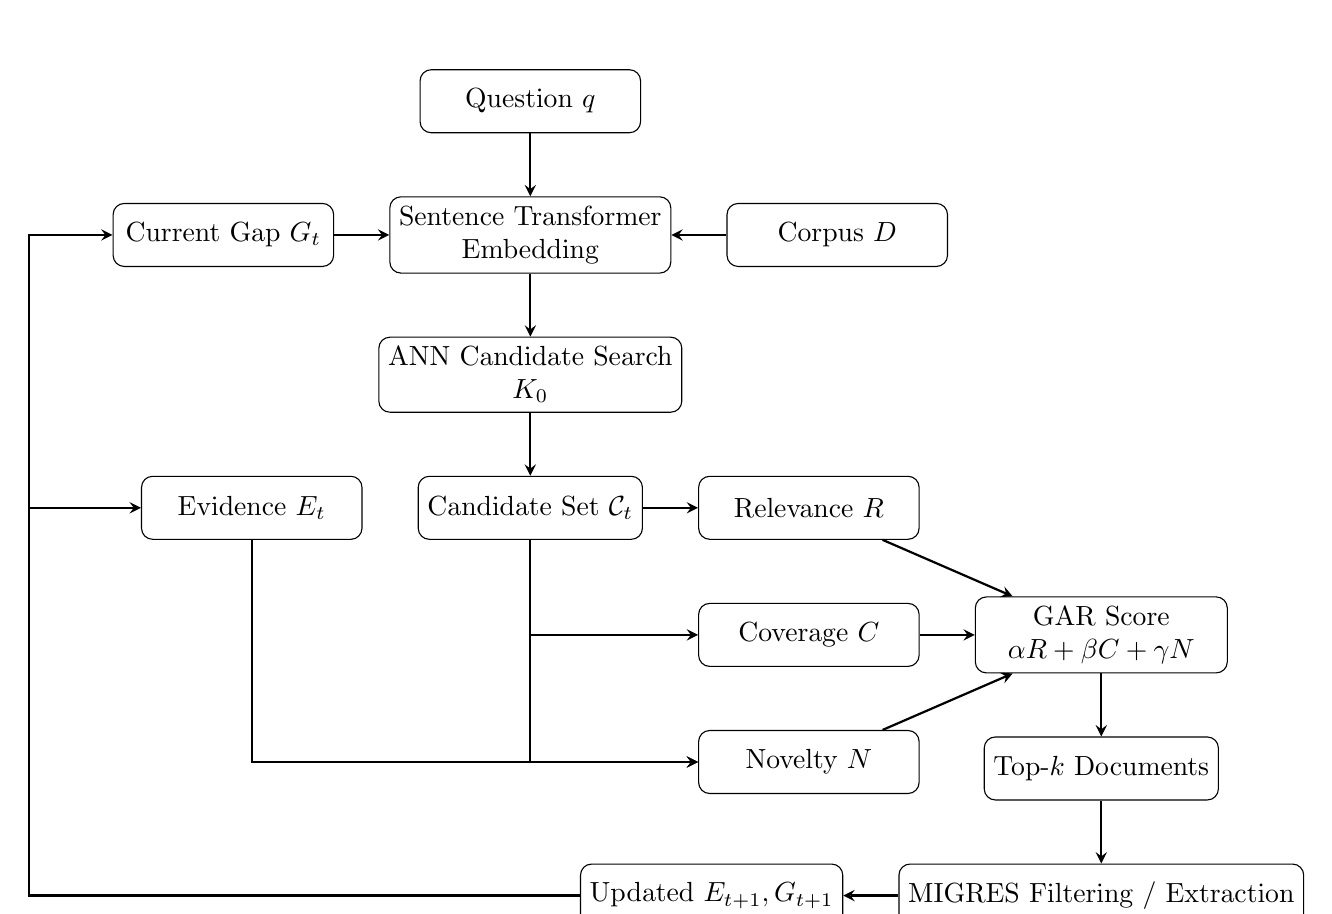
\begin{tikzpicture}[node distance=8mm and 7mm]

% Inputs
\node[block] (q) {Question $q$};

% Embedding and candidate generation
\node[important,below=of q] (emb) {Sentence Transformer\\Embedding};
\node[block,left=of emb] (g) {Current Gap $G_t$};
\node[block,right=of emb] (d) {Corpus $D$};
\node[important,below=of emb] (ann) {ANN Candidate Search\\$K_0$};
\node[block,below=of ann] (cand) {Candidate Set $\mathcal{C}_t$};
\node[block,left=of cand] (e) {Evidence $E_t$};

% GAR components
\node[block,right=of cand] (r) {Relevance $R$};
\node[block,below=of r] (c) {Coverage $C$};
\node[block,below=of c] (n) {Novelty $N$};

% Final score
\node[important,right=of c] (score)
    {GAR Score\\$\alpha R+\beta C+\gamma N$};

% Output and MIGRES
\node[block,below=of score] (top) {Top-$k$ Documents};
\node[block,below=of top] (mig) {MIGRES Filtering / Extraction};
\node[block,left=of mig] (next) {Updated $E_{t+1},G_{t+1}$};

% Input arrows
\draw[arrow] (q) -- (emb);
\draw[arrow] (g) -- (emb);
\draw[arrow] (d) -- (emb);

% Embedding -> ANN -> candidates
\draw[arrow] (emb) -- (ann);
\draw[arrow] (ann) -- (cand);

% Candidate -> each GAR component
\draw[arrow] (cand) -- (r);
\draw[arrow] (cand) |- (c);
\draw[arrow] (cand) |- (n);

% Evidence affects novelty
\draw[arrow] (e) |- (n);

% Components -> final score
\draw[arrow] (r) -- (score);
\draw[arrow] (c) -- (score);
\draw[arrow] (n) -- (score);

% Final retrieval -> MIGRES
\draw[arrow] (score) -- (top);
\draw[arrow] (top) -- (mig);

% MIGRES updates the state
\draw[arrow] (mig) -- (next);

% Feedback loop for next iteration
\draw[arrow] (next.west) -- ++(-7,0) |- (g.west);
\draw[arrow] (next.west) -- ++(-7,0) |- (e.west);

\end{tikzpicture}

\caption{GAR methodology within the MIGRES framework.}
\label{fig:gar-architecture}

\end{figure}
\clearpage

\subsection{Flow Diagram}
The flow diagram presents the iterative execution of the proposed method. 
After each retrieval and evidence-extraction step, MIGRES updates the 
information state. GAR then performs the next retrieval until the stopping 
condition is satisfied.
\begin{figure}[H]
\centering
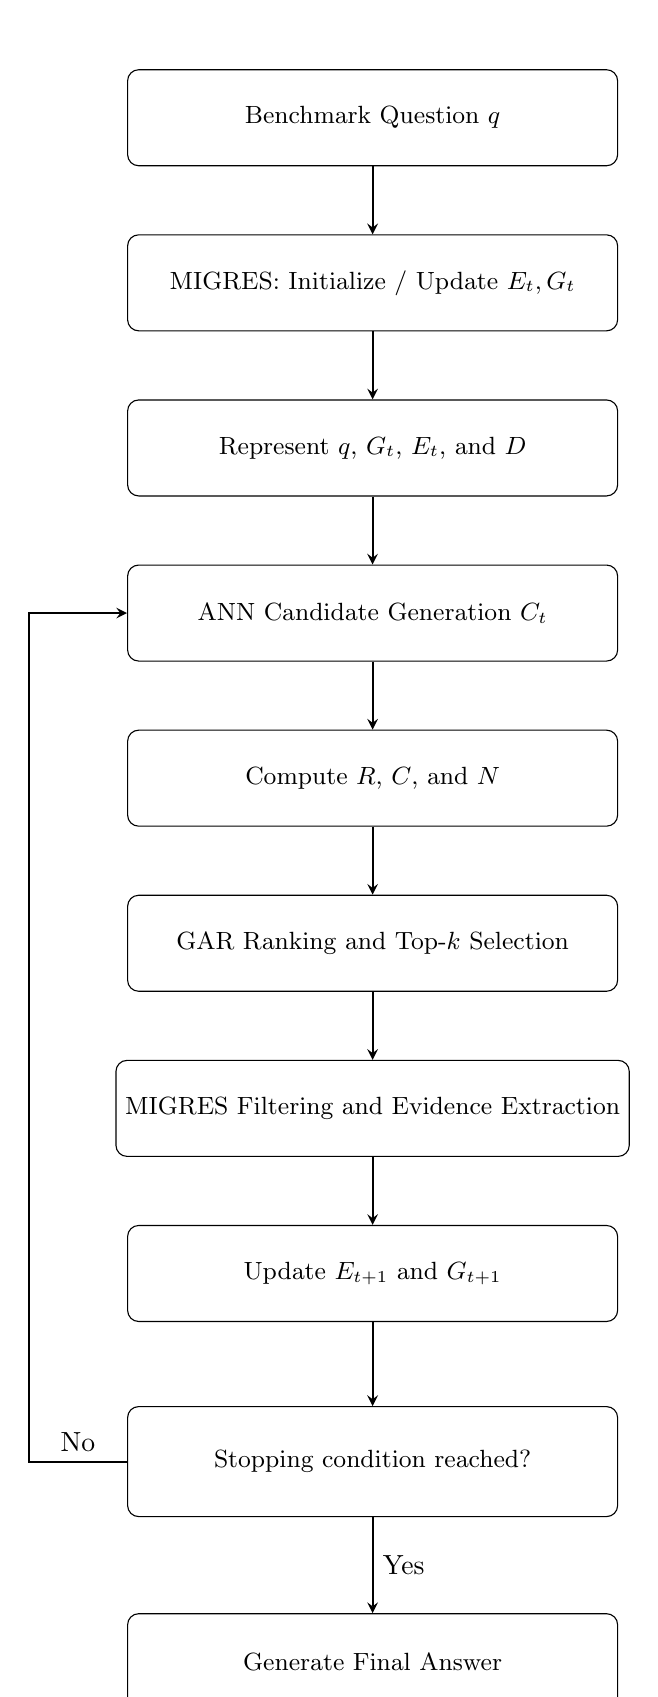
\begin{tikzpicture}[
    node distance=0.34in,
    flowbox/.style={draw, rounded corners, align=center, minimum width=2.45in, minimum height=0.48in, font=\small},
    decision/.style={draw, rounded corners, align=center, minimum width=2.45in, minimum height=0.55in, font=\small},
    arrow/.style={->, >=stealth, line width=0.7pt}
]
\node[flowbox] (question) {Benchmark Question $q$};
\node[flowbox, below=of question] (state) {MIGRES: Initialize / Update $E_t,G_t$};
\node[flowbox, below=of state] (repr) {Represent $q$, $G_t$, $E_t$, and $D$};
\node[flowbox, below=of repr] (candidate) {ANN Candidate Generation $C_t$};
\node[flowbox, below=of candidate] (score) {Compute $R$, $C$, and $N$};
\node[flowbox, below=of score] (rank) {GAR Ranking and Top-$k$ Selection};
\node[flowbox, below=of rank] (extract) {MIGRES Filtering and Evidence Extraction};
\node[flowbox, below=of extract] (update) {Update $E_{t+1}$ and $G_{t+1}$};
\node[decision, below=0.42in of update] (stop) {Stopping condition reached?};
\node[flowbox, below=0.48in of stop] (answer) {Generate Final Answer};

\draw[arrow] (question) -- (state);
\draw[arrow] (state) -- (repr);
\draw[arrow] (repr) -- (candidate);
\draw[arrow] (candidate) -- (score);
\draw[arrow] (score) -- (rank);
\draw[arrow] (rank) -- (extract);
\draw[arrow] (extract) -- (update);
\draw[arrow] (update) -- (stop);
\draw[arrow] (stop) -- node[right]{Yes} (answer);
\draw[arrow] (stop.west) -- ++(-1.25,0) node[above,midway]{No} |- (candidate.west);
\end{tikzpicture}
\caption{Operational flow of the proposed GAR-based iterative retrieval solution.}
\label{fig:gar-flow}
\end{figure}
\clearpage
\section{Mathematical Formulation}

At each retrieval iteration $t$, GAR receives the question $q$, the previously collected evidence $E_t$, the current missing-information requirements $G_t=\{g_1,\ldots,g_m\}$, and the document corpus $D$:

\[
(q,E_t,G_t,D).
\]

Here, $q$ represents the original question, $E_t$ represents the evidence collected so far, $G_t$ represents the information that is still missing, and $D$ is the searchable document collection. The information gap and evidence are provided by the surrounding iterative retrieval process.

GAR uses a fixed sentence-embedding function $\phi(x)$ to represent questions, gaps, documents, and evidence as vectors. The primary configuration uses \textbf{sentence-transformers/multi-qa-mpnet-base-cos-v1} \cite{reimers2019sentence,st2020mpnet}. The similarity between two text items is measured using cosine similarity:

\[
s(x,y)=
\frac{1}{2}
\left(
1+
\frac{\phi(x)^T\phi(y)}
{\|\phi(x)\|_2\|\phi(y)\|_2}
\right).
\]

This normalizes the similarity score to the range $[0,1]$.

Before ranking, GAR creates a candidate set using approximate nearest-neighbor (ANN) search:

\[
C_t =
\operatorname{ANN}_{K_0}(q,D)
\cup
\bigcup_{i=1}^{m}
\operatorname{ANN}_{K_0}(g_i,D),
\]

where $K_0$ is the number of candidate documents retrieved for scoring. Duplicate documents are removed from $C_t$.

GAR then evaluates each candidate using three scores. First, gap relevance measures how relevant a document is to both the question and the current information gap. With equal gap weights, it is defined as:

\[
R(d,q,G_t)
=
\lambda s(d,q)
+
(1-\lambda)
\frac{1}{m}
\sum_{i=1}^{m}s(d,g_i),
\]

where $0\leq\lambda\leq1$ controls the balance between the original question and the information gap.

Second, gap coverage measures how much of the missing information is covered by a document. Using normalized content tokens $\tau(\cdot)$:

\[
C(d,G_t)
=
\frac{1}{m}
\sum_{i=1}^{m}
\frac{|\tau(d)\cap\tau(g_i)|}
{|\tau(g_i)|}.
\]

This score lies between $0$ and $1$. Empty gap requirements are removed before this calculation.

Third, evidence novelty measures how different a candidate document is from the evidence already collected:

\[
N(d,E_t)
=
1-\max_{e\in E_t}s(d,e).
\]

A document that is highly similar to existing evidence receives a lower novelty score. At the first iteration, where $E_0=\emptyset$, novelty is set to $1$.

The three scores are combined into the final GAR score:

\[
S(d\mid q,E_t,G_t)
=
\alpha R(d,q,G_t)
+
\beta C(d,G_t)
+
\gamma N(d,E_t),
\]

where

\[
\alpha,\beta,\gamma\geq0,
\qquad
\alpha+\beta+\gamma=1.
\]

The weights determine the importance of relevance, coverage, and novelty, respectively. Since all three component scores are normalized, the final GAR score also lies between $0$ and $1$.

Finally, GAR ranks the candidate documents according to their scores and returns the top-$k$ documents:

\[
T_t=
\operatorname{TopK}_{d\in C_t}
S(d\mid q,E_t,G_t).
\]

The selected documents are then used in the next iteration, where the evidence and missing-information state may be updated before GAR performs the next retrieval.
\clearpage
\section{Datasets and Model}

\subsection{Datasets}

The evaluation uses six question-answering datasets that involve multi-hop reasoning, information gathering, or retrieval from supporting evidence. These datasets provide different types of information-seeking tasks and allow the proposed retrieval approach to be evaluated across varied retrieval and reasoning requirements.

The datasets used in this study are:

\begin{itemize}
    \item \textbf{WikiHop:} A multi-document question-answering dataset that requires information to be combined across multiple documents \cite{welbl2018wikihop}.

    \item \textbf{HotpotQA:} A multi-hop question-answering dataset with supporting facts. The FullWiki setting is used to evaluate retrieval from a larger Wikipedia corpus \cite{yang2018hotpotqa}.

    \item \textbf{MuSiQue:} A multi-hop question-answering dataset designed for compositional reasoning, with questions requiring two to four reasoning hops \cite{trivedi2022musique}.

    \item \textbf{Natural Questions:} A question-answering dataset based on real search queries, with annotations derived from Wikipedia \cite{kwiatkowski2019natural}.

    \item \textbf{TriviaQA:} A question-answering dataset containing questions paired with independently collected evidence documents \cite{joshi2017triviaqa}.

    \item \textbf{StrategyQA:} A question-answering dataset that requires implicit reasoning and uses supporting Wikipedia evidence \cite{geva2021strategyqa}.
\end{itemize}

Where official splits are available, the training, validation, and test sets are kept separate. The validation set is used for GAR hyperparameter selection, while the test set is reserved for final evaluation.

\subsection{Model}

GAR uses a Sentence Transformer model to convert questions, information gaps, documents, and collected evidence into numerical vector representations. Sentence Transformers are designed to generate embeddings that capture the semantic meaning of text, allowing text items to be compared based on semantic similarity rather than only exact word matching.

The primary model used in this study is \texttt{multi-qa-mpnet-base-cos-v1} from Sentence Transformers. It produces 768-dimensional dense embeddings and is designed for semantic search \cite{reimers2019sentence,st2020mpnet}. The same model is used for questions, gap requirements, documents, and evidence to maintain a consistent representation throughout the retrieval process.

\section{Baseline Comparison}

The proposed method is compared with established retrieval approaches to evaluate its effectiveness. The main retrieval systems are summarized in Table~\ref{tab:baseline-comparison}.

\begin{table}[H]
\centering
\caption{Retrieval baseline comparison}
\label{tab:baseline-comparison}
\renewcommand{\arraystretch}{1.25}
\begin{tabular}{|p{1.55in}|p{1.45in}|p{3.05in}|}
\hline
\textbf{System} & \textbf{Retrieval type} & \textbf{Role} \\ \hline
MIGRES+BM25 & Sparse lexical & Main baseline \cite{robertson2009bm25} \\ \hline
MIGRES+DPR & Dense bi-encoder & Supervised dense baseline \cite{karpukhin2020dpr} \\ \hline
MIGRES+Contriever & Unsupervised dense & Contrastive-learning dense baseline \cite{izacard2022contriever} \\ \hline
MIGRES+ColBERTv2 & Late interaction & Multi-vector retrieval baseline \cite{santhanam2022colbertv2} \\ \hline
MIGRES+SPLADE & Neural sparse & Neural sparse baseline \cite{formal2021splade} \\ \hline
MIGRES+GAR & Gap-aware & Proposed retrieval method \\ \hline
\end{tabular}
\end{table}

For a fair comparison, the same dataset splits, questions, document corpus, retrieval depth $k$, and other system settings are used for all methods wherever possible. Only the retrieval method is changed. The baseline methods are used with their standard implementations and settings.

\section{Experimental Design}

The experiments are conducted in four main stages. First, the GAR hyperparameters are selected using the validation set. The selected configuration is then fixed and used for the main comparison with existing retrieval methods. Ablation experiments are then performed to study the contribution of the individual GAR components. Finally, the effect of the ANN candidate-pool size is analyzed.

\subsection{Hyperparameter Selection}

GAR uses five hyperparameters: $\alpha$, $\beta$, $\gamma$, $\lambda$, and $K_0$. The roles of these parameters are shown in Table~\ref{tab:gar-hyperparameters}.

\begin{table}[H]
\centering
\caption{GAR hyperparameters}
\label{tab:gar-hyperparameters}
\renewcommand{\arraystretch}{1.25}
\begin{tabular}{|p{1.05in}|p{1.55in}|p{3.65in}|}
\hline
\textbf{Parameter} & \textbf{Role} & \textbf{Description} \\ \hline
$\alpha$ & Relevance weight & Controls the importance of relevance. \\ \hline
$\beta$ & Coverage weight & Controls the importance of coverage. \\ \hline
$\gamma$ & Novelty weight & Controls the importance of new information. \\ \hline
$\lambda$ & Question weight & Controls the importance of the original question. \\ \hline
$K_0$ & Candidate-pool size & Controls the number of candidate documents. \\ \hline
\end{tabular}
\end{table}

The validation set is used to select the GAR configuration:

\[
\theta_{\mathrm{GAR}}
=
\{\alpha,\beta,\gamma,\lambda,K_0\}.
\]

Bayesian optimization is used to search for the configuration that gives the best validation performance \cite{snoek2012practical}. Recall@k is used as the primary validation metric. The search includes different values of $\alpha$, $\beta$, $\gamma$, and $\lambda$, while $K_0$ is selected from the predefined values:

\[
K_0\in\{50,100,200,500\}.
\]

The best configuration is selected from the validation results and then fixed for the remaining experiments. The test set is not used to change the selected hyperparameters.

\subsection{Main Comparison}

After the GAR configuration is fixed, the main experiment compares GAR with established retrieval methods. The methods evaluated are BM25, DPR, Contriever, ColBERTv2, and SPLADE.

All methods use the same datasets, questions, document corpus, and final retrieval depth $k$ wherever possible. This allows the comparison to focus on the difference between the retrieval methods.

The main evaluation measures retrieval performance and downstream answer quality.

\subsection{Ablation Study}

An ablation study is conducted to determine the contribution of the three main GAR components: relevance, coverage, and novelty.

The complete GAR score is:

\[
S_{\mathrm{GAR}}=\alpha R+\beta C+\gamma N.
\]

Each component is removed separately to create three variants:

\[
S_{-R}=\beta C+\gamma N,
\] \[
S_{-C}=\alpha R+\gamma N,
\] \[
S_{-N}=\alpha R+\beta C.
\]

The results of these variants are compared with the complete GAR model to determine the contribution of each component.

\subsection{Candidate-Pool Analysis}

The effect of the ANN candidate-pool size $K_0$ is also evaluated. The following values are considered:

\[
K_0\in\{50,100,200,500\}.
\]

The different settings are compared based on retrieval performance and latency. The validation results are used to select the final $K_0$, which is then fixed for the test evaluation.

\subsection{Evaluation Metrics}

\subsubsection{Retrieval Evaluation}

We evaluate retrieval using Recall@k, Precision@k, MRR, and nDCG@k. Recall@k measures how much relevant evidence is retrieved, while Precision@k measures how many retrieved documents are relevant. MRR measures how early the first relevant document appears, and nDCG@k evaluates the quality of the ranking. Evidence coverage is also reported where suitable annotations are available.

\subsubsection{Downstream Answer Evaluation}

Final answer quality is measured using the official dataset metrics, including Exact Match (EM), token-level F1, classification accuracy, and supporting-evidence quality where applicable.

\subsubsection{Efficiency Evaluation}

Efficiency is evaluated using retrieval latency, ANN indexing time, index memory, number of retrieval iterations, and number of documents scored. LLM calls, token usage, and API cost are also recorded where applicable.

\subsubsection{Statistical Analysis}

We report effect sizes and confidence intervals. Since all methods are evaluated on the same questions, paired bootstrap or paired permutation testing is used to determine whether performance differences are statistically significant.

\section{Experimental Environment and Reproducibility}

The experiments use a software environment that supports dataset preparation, sentence embedding, ANN indexing, GAR retrieval, and evaluation. The exact software versions, hardware configuration, and model settings used in the experiments are recorded.

For reproducibility, the datasets, document corpus, models, GAR parameters, ANN settings, and software versions used in the experiments are recorded. The same data and evaluation settings are used for all retrieval methods. The GAR parameters selected during validation are fixed before the final test.

The experimental pipeline is:

\[
\text{Dataset}
\rightarrow
\text{MIGRES State}
\rightarrow
\text{GAR Retrieval and Ranking}
\rightarrow
\text{Evidence Update}
\rightarrow
\text{Evaluation}.
\]
\clearpage
\section{Chapter Solution Summary}

This chapter presented the proposed Gap-Aware Retrieval (GAR) approach for iterative document retrieval. GAR considers the original question, the current information gap, and previously collected evidence to select relevant and less redundant documents.

The chapter described the GAR architecture, retrieval process, mathematical formulation, and experimental design. GAR will evaluated against established retrieval methods using controlled experiments, with hyperparameters selected on the validation set before final test evaluation. Ablation and efficiency analyses are also included to examine the contribution and practical performance of the proposed approach.

Overall, the methodology provides a complete framework for implementing and evaluating GAR for iterative information retrieval.

\clearpage

% ============================================================
% CHAPTER 6
% SOFTWARE AND HARDWARE REQUIREMENTS
% ============================================================

\setcounter{table}{0}
\renewcommand{\thetable}{6.\arabic{table}}

\addcontentsline{toc}{chapter}{6. SOFTWARE AND HARDWARE REQUIREMENTS}

\chaptertitle{6}{SOFTWARE AND HARDWARE REQUIREMENTS}

\justifying

The proposed solution requires a Python-based environment for dataset preparation, embedding generation, vector search, GAR retrieval and ranking, hyperparameter selection, and evaluation. Jupyter Notebook is used for experiment development and analysis, while LaTeX is used for preparing the research document. The main software and hardware requirements are described below.

\subsection*{6.1 Software Requirements}

The main software tools required for the implementation are shown in Table~\ref{tab:software-requirements}.

\begin{table}[H]
\centering
\caption{Software requirements}
\label{tab:software-requirements}
\renewcommand{\arraystretch}{1.2}
\begin{tabular}{|p{1.65in}|p{1.45in}|p{2.95in}|}
\hline
\textbf{Software / Tool} & \textbf{Version} & \textbf{Purpose} \\ \hline
Python & 3.14.7 & Main programming environment for GAR implementation, data processing, retrieval, and evaluation. \\ \hline
Jupyter Notebook & 7.6.2 & Experiment development, execution, and result analysis. \\ \hline
PyTorch & 2.13.0 & Tensor computation and neural model execution. \\ \hline
Sentence Transformers & 5.6.1 (model: multi-qa-mpnet-base-cos-v1) & Generates semantic embeddings for questions, documents, gaps, and evidence. \\ \hline
Pinecone & Client v9.1.0 (API 2025-10) & Stores document embeddings and performs vector similarity search for candidate retrieval. \\ \hline
Bayesian Optimization Library & 3.3.0 (bayesian-optimization) & Optimizes GAR hyperparameters on the validation set. \\ \hline
LaTeX & Overleaf & Preparation of the research document. \\ \hline
\end{tabular}
\end{table}

The primary embedding model is \texttt{multi-qa-mpnet-base-cos-v1} from Sentence Transformers. It is used to generate a common semantic representation for questions, information gaps, documents, and collected evidence. The model remains fixed and is not fine-tuned during the primary experiments.
\clearpage
\subsection*{6.2 Modules Description}

The proposed GAR methodology is divided into three major modules: 
the Retrieval Module, the Scoring Module, and the Selection Module. 
The responsibilities of each module are described in Table~\ref{tab:module-description}.

\begin{table}[H]
\centering
\caption{Modules Description}
\label{tab:module-description}
\renewcommand{\arraystretch}{1.25}
\begin{tabular}{|p{1.65in}|p{4.4in}|}
\hline
\textbf{Module} & \textbf{Responsibility} \\ \hline

Retrieval Module &
Generates embeddings for the question, current information gap, and document corpus using the Sentence Transformer model. It then performs Approximate Nearest Neighbor (ANN) search to generate the candidate document set $C_t$. \\ \hline

Scoring Module &
Evaluates the candidate documents using three signals: relevance, gap coverage, and evidence novelty. These scores are combined using the GAR scoring function $S(d \mid q,E_t,G_t) = \alpha R + \beta C + \gamma N$. \\ \hline

Selection Module &
Ranks the candidate documents according to their GAR scores and selects the Top-$k$ documents. The selected documents are passed to MIGRES for filtering and extraction, after which the updated evidence $E_{t+1}$ and information gap $G_{t+1}$ are used for the next retrieval iteration. \\ \hline

\end{tabular}
\end{table}

\clearpage
% ============================================================
% CHAPTER 7
% APPLICATIONS
% ============================================================

\addcontentsline{toc}{chapter}{7. APPLICATIONS}

\chaptertitle{7}{APPLICATIONS}

\begin{enumerate}[
    leftmargin=0.30in,
    itemsep=0.12in
]

\item
\textbf{Multi-Hop Question Answering:}
The methodology is suited to questions whose answers require complementary information from multiple documents or retrieval steps.

\item
\textbf{Iterative Retrieval-Augmented Generation:}
GAR can serve as a retrieval component in RAG systems that repeatedly acquire evidence as the answer is developed and the information requirement changes.

\item
\textbf{Research-Oriented Evidence Retrieval:}
The gap and evidence signals can help research-oriented systems focus subsequent retrieval on information that is still required rather than repeatedly collecting already-covered material.

\item
\textbf{Large-Scale Evidence Gathering:}
ANN candidate generation allows the retrieval stage to operate over large document collections while restricting full GAR scoring to a manageable candidate set.

\item
\textbf{Missing-Information-Guided AI Systems:}
The approach is applicable to systems that explicitly maintain an information-gap state and can provide that state to the retrieval component.

\end{enumerate}

\clearpage

% ============================================================
% CHAPTER 8
% GANTT CHART
% ============================================================

\setcounter{table}{0}
\renewcommand{\thetable}{8.\arabic{table}}


\addcontentsline{toc}{chapter}{8. GANTT CHART}

\chaptertitle{8}{GANTT CHART}

\begin{center}

\textbf{Figure 6.1: Gantt Chart}

\vspace{0.15in}

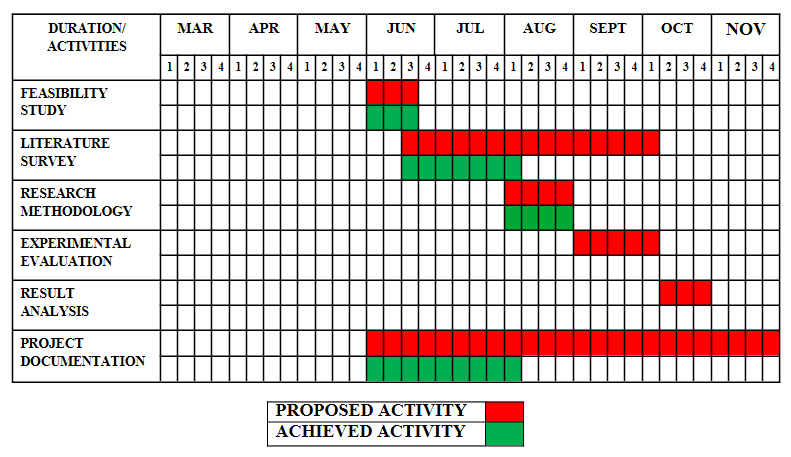
\includegraphics[width=0.95\textwidth]{gantt_chart.png}

\end{center}
\clearpage

% ============================================================
% CHAPTER 9
% CONCLUSION
% ============================================================

\addcontentsline{toc}{chapter}{9. CONCLUSION}

\chaptertitle{9}{CONCLUSION}

\justifying

This methodology presents a controlled approach for evaluating Gap-Aware Retrieval (GAR) within the MIGRES framework. GAR uses the current information gap and previously collected evidence to retrieve and rank documents based on relevance, coverage, and novelty. The selected documents are then passed to MIGRES for filtering, extraction, and further iteration.

GAR is evaluated against established retrieval methods, including BM25, DPR, Contriever, ColBERTv2, and SPLADE. Ablation studies are used to examine the contribution of each GAR component, while retrieval quality, answer quality, and efficiency are evaluated using predefined metrics.

Overall, the methodology is designed to determine whether using the information gap and existing evidence can improve retrieval in iterative information-seeking systems while keeping the surrounding framework unchanged.

\clearpage

% ============================================================
% REFERENCES
% ============================================================

\addcontentsline{toc}{chapter}{REFERENCES}

\fronttitle{REFERENCES}

\renewcommand{\bibname}{}

\bibliographystyle{IEEEtran}
\bibliography{citation}

\end{document}
